\documentclass{article}
\usepackage{graphicx}
\begin{document}
\section{Discrete Cmac}
\subsection{Description}
\subsection{Results}
  \paragraph{Generalization Vs Convergence:}
  Refer to the "Data/ConvergenceVsGeneralization" folder for graphs. Clearly,
  as the generalization number increases, the model has a hard time converging.This can
  be attributed to the fact that generalization number,g indicates to a degree the similarity
  between tasks. As the g increases, unrelated tasks are grouped as similar and the model tends
  to overfit. Ideally, g is chosen so that tasks which are related have similar value whiles tasks
  which are different have clear cut distinct values. 
  \paragraph{Accuracy:}
    Below is a graph that depicts the accuray of the Discrete Cmac
  \begin{figure}[h!]
    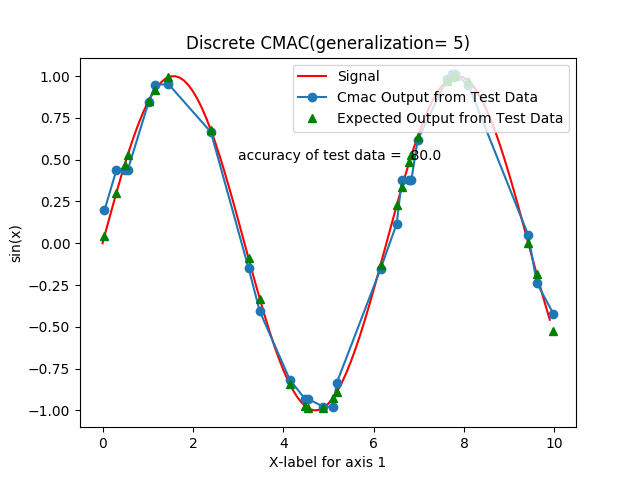
\includegraphics[scale=0.65]{./Data/Accuracy/discreteAccuracy.png}
  \end{figure}

\section{Continous Cmac}
\subsection{Description}
\subsection{Results}
  \paragraph{Accuracy:}
    Below is a graph that depicts the accuray of the Continous Cmac
  \begin{figure}[h]
     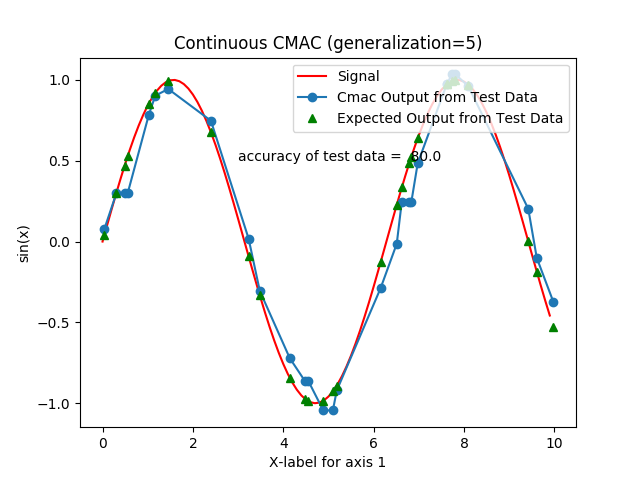
\includegraphics[scale=0.65]{./Data/Accuracy/continousAccuracy.png}
  \end{figure}
  \paragraph{Discrete Vs Continous Cmac:}
\section{Recurrent Networks}
\end{document}


